%Este trabalho está licenciado sob a Licença Atribuição-CompartilhaIgual 4.0 Internacional Creative Commons. Para visualizar uma cópia desta licença, visite http://creativecommons.org/licenses/by-sa/4.0/deed.pt_BR ou mande uma carta para Creative Commons, PO Box 1866, Mountain View, CA 94042, USA.

\documentclass[12pt]{article}

\input ../preambulo.tex

\lstset {
  language=C++,
}

\makeindex

\begin{document}

\title{Minicurso de C/C++ para Matemática}
\author{Pedro H A Konzen}
\date{\today}
% \ifishtml
% \else
% \addcontentsline{toc}{chapter}{Capa}
% \fi

\maketitle

%references
\nocite{}

\tableofcontents

\section{Licença}\label{sec_licenca}
%\addcontentsline{toc}{Section}{Licença}

Este trabalho está licenciado sob a Licença Atribuição-CompartilhaIgual 4.0 Internacional Creative Commons. Para visualizar uma cópia desta licença, visite http://creativecommons.org/licenses/by-sa/4.0/deed.pt\_BR ou mande uma carta para Creative Commons, PO Box 1866, Mountain View, CA 94042, USA.


\section{Sobre a Linguagem}\label{sec_sobrepy}

\hl{C e C++ são \emph{linguagens} de programação \emph{compiladas} de propósito geral}. \hl{A primeira é \emph{estruturada e procedural}}, tendo sido crada em 1972 por Dennis Ritchie\footnote{Dennis Ritchie, 1941-2011, cientista da computação estadunidense. Fonte: \href{https://pt.wikipedia.org/wiki/Dennis_Ritchie}{Wikipédia}.}. A segunda foi inicialmente desenvolvida por Bjarne Stroustrup\footnote{Bjarne Stroustrup, 1950, cientista da computação dinamarquês. Fonte: \href{https://pt.wikipedia.org/wiki/Bjarne_Stroustrup}{Wikipédia}.} como uma extensão da primeira. Em sua mais recente especificação, a \hl{linguagem C++ se caracteriza por ser \emph{multi-paradigma} (\emph{imperativa}, \emph{orientada a objetos} e \emph{genérica})}.

\subsection{Instalação e Execução}

\hl{Códigos C/C++ precisam ser compilados antes de serem executados}. De forma simplificada, o \emph{compilador} é um programa que interpreta e converte o código em um programa executável em computador. Há vários compiladores gratuitos disponíveis na web. Ao longo deste minicurso, usaremos a coleção de compiladores \href{https://gcc.gnu.org/}{GNU GCC} instalados em sistema operacional {\linux}.

\subsubsection{IDE}

\hl{Usar um \emph{ambiente integrado de desenvolvimento} (IDE, em inglês, \textit{integrated development environment}) é a melhor forma de capturar o melhor das linguagens C/C++}. Algumas alternativas são:
\begin{itemize}
\item \href{https://www.eclipse.org/ide/}{Eclipse}
\item \href{https://www.gnu.org/software/emacs/download.html}{GNU Emacs}
\item \href{https://code.visualstudio.com/}{VS Code}
\end{itemize}

\subsection{Olá, mundo!}

Vamos \hl{implementar} nosso primeiro programa C/C++. \hl{Em geral, são três passos: 1. escrever; 2. compilar; 3. executar.}

\begin{enumerate}[1.]
\item \hlemph{Escrever o código}.

  Em seu IDE preferido, digite o código:
\begin{lstlisting}[caption=ola.cc, label=cod:ola]
#include <stdio.h>

int main()
{
  printf("Olá, mundo!\n");
  return 0;
}
\end{lstlisting}
  
\item \hlemph{Compilar}.

Para compilá-lo, digite no terminal de seu sistema operacional
\begin{lstlisting}
$ gcc ola.cc -o ola.x
\end{lstlisting}

\item \hlemph{Executar}.

Terminada a compilação, o arquivo executável \lstinline+ola.x+ é criado. Para executá-lo, digite
\begin{lstlisting}
$ ./ola.x
\end{lstlisting}  
\end{enumerate}


\section{Elementos da Linguagem}\label{sec_elem}

\subsection{Tipos de Dados Básicos}

\hl{Na linguagem C/C++, \emph{dados} são alocados em \emph{variáveis} com tipos declarados}\footnote{Consulte \href{https://en.wikipedia.org/wiki/C_data_types}{Wikipedia: C data type} para uma lista dos tipos de dados disponíveis na linguagem}.

\begin{ex}
  Consideramos o seguinte código.
\begin{lstlisting}[caption=dados.cc]
/* dados.cc
   Exemplo de alocação de variáveis.
*/
#include <stdio.h>

int main() 
{
  // var inteira
  int i = 1;
  // var pto flutuante
  double x;

  x = 2.5;
  char s[6] = "i + x";
  double y = i + x;
  printf("%s = %f\n", s, y);
  return 0;
}
\end{lstlisting}

  Na linha 9, é alocada uma \hlemph{variável do tipo inteira} com \emph{identificador} \lstinline+i+ e \emph{valor} \lstinline+1+. Na linha 11, é alocada uma \hlemph{variável do tipo ponto flutuante} (64~\textit{bits}) com identificador \lstinline+x+.

  Na linha 14, é alocada uma \hlemph{variável do tipo \textit{string}}\footnote{Um arranjo de \lstinline+char+ (caracteres).}. Na linha 15, alocamos uma nova variável \lstinline+y+.
\end{ex}

\begin{obs}\normalfont{(\hl{Comentários e Continuação de Linha}.)}
  Códigos C++ admitem \emph{comentários} e \emph{continuação de linha} como no seguinte exemplo acima. Comentários em linha podem ser feitos com \lstinline+\\+ e de múltiplas linhas com \lstinline+\* ... */+. Linhas de instruções muito compridas podem ser quebradas em múltiplas linhas com a instrução de continuação de linha \lstinline+\+.
\end{obs}

\begin{obs}\normalfont{(\hl{Notação científica}.)}
  Podemos usar \emph{notação científica} em C++. Por exemplo $5.2\times 10^{-2}$ é digitado da seguinte forma \lstinline+5.2e-2+.

\begin{lstlisting}[caption=notacaoCientifica.cpp]
#include <stdio.h>

int main()
{

  int i = -51;
  double x = 5.2e-2;

  // inteiro
  printf("inteiro: %d\n", i);
  // fixada
  printf("fixada: %f\n", x);
  // notação científica
  printf("científica: %e\n", x);
  return 0;
}
\end{lstlisting}
\end{obs}

\begin{exr}
  Antes de implementar, diga qual o valor de \lstinline+x+ após as seguintes instruções.
\begin{lstlisting}
int x = 1;
int y = x;
y = 0;
\end{lstlisting}
  Justifique seu resposta e verifique-a.
\end{exr}

\begin{exr}
  Implemente um código em que a(o) usuária(o) entra com valores para as variáveis \lstinline+x+ e \lstinline+y+. Então, os valores das variáveis são permutados entre si. Dica: a entrada de dados por usuária(o) pode ser feita com o método C/C++ \href{https://cplusplus.com/reference/cstdio/scanf}{scanf} da biblioteca \href{https://cplusplus.com/reference/cstdio}{stdio.h}. Por exemplo,
\begin{lstlisting}
double x;
scanf("%lf", x);
\end{lstlisting}
faz a leitura de um \lstinline+double+ (long float) e o armazena na variável \lstinline+x+.
\end{exr}

\subsection{Operações Aritméticas Elementares}

Os operadores aritméticos elementares são\footnote{Em ordem de precedência.}:
\begin{itemize}
\item[]\hl{{\lstinline!*!}, {\lstinline!/!}, {\texttt{\%}} \emph{: multiplicação, divisão, módulo}}
\item[]\hl{{\lstinline!+!}, {\lstinline!-!} \emph{: adição, subtração}}
\end{itemize}

\begin{ex}
  Qual é o valor impresso pelo seguinte código?
\begin{lstlisting}
#include <stdio.h>

int main()
{
  printf("%f\n", 2+17%9/2*2-1 );
  return 0;
}
\end{lstlisting}

  Observamos que as operações {\lstinline+*+}, {\lstinline+/+} e {\texttt{\%}} têm precedência maior que as operações {\lstinline!+!} e {\lstinline!-!}. Operações de mesma precedência seguem a ordem da esquerda para direita, conforme escritas na linha de comando. \hl{Usa-se parênteses para alterar a precedência entre as operações}, por exemplo
\begin{lstlisting}
printf("%f\n", (2+17)%9/2*2-1 );
\end{lstlisting}
imprime o resultado \lstinline!-1!. Sim, pois a \hl{divisão inteira} está sendo usada. Para computar a divisão em ponto flutuante, um dos operandos deve ser \lstinline!double!. Para tanto, podemos fazer um \hlemph{\textit{casting}} \lstinline!double((2+17)\%9)/2*2-1! ou, simplesmente, \lstinline!(2+17)\%9/2.*2-1!.
\end{ex}

\begin{obs}\normalfont{(\hl{Precedência das Operações}.)}
Consulte mais informações sobre a precedência de operadores em \href{https://en.wikipedia.org/wiki/Operators_in_C_and_C\%2B\%2B#Operator_precedence}{Wikipedia:Operators in C and C++}.
\end{obs}

\begin{exr}
  Escreva um programa para computar o vértice da parábola
  \begin{equation}
    ax^2 + bx + c = 0,
  \end{equation}
  para $a = 2$, $b = -2$ e $c = 4$. 
\end{exr}

\hl{O operador {\lstinline+\%+} módulo computa o \emph{resto} da divisão inteira}, por exemplo, \lstinline+5\%2+ é igual a \lstinline+1+.

\begin{exr}
  Use C/C++ para computar os inteiros não negativos $q$ e $r$ tais que
  \begin{equation}
    25 = q\cdot 3 + r,
  \end{equation}
  sendo $r$ o menor possível.
\end{exr}

\subsection{Funções e Constantes Elementares}

\hl{A \emph{biblioteca} C/C++ {\href{https://cplusplus.com/reference/cmath}{math.h}} disponibiliza várias funções e constantes elementares}.
\begin{lstlisting}[caption=mat.cc]
#include <stdio.h>
#include <math.h>

int main()
{
  printf("pi = %.9e\n", M_PI);
  printf("2^(1/2) = %.5f\n", sqrt(2.));
  printf("log(e) = %f\n", log(M_E));
  return 0;
}
\end{lstlisting}

\begin{obs}\normalfont{(\hl{Logaritmo Natural}.)}
  Notamos que \lstinline+log+ é a função logaritmo natural, i.e. $\ln(x) = \log_e(x)$. A implementação C/C++ para o logaritmo de base 10 é \lstinline!log10(x)!.
\end{obs}

\begin{exr}
  Compute
  \begin{enumerate}[a)]
  \item $\displaystyle \sen\left(\frac{\pi}{4}\right)$
  \item $\displaystyle \log_3(\pi)$
  \item $\displaystyle e^{\log_2(\pi)}$
  \item $\displaystyle \sqrt[3]{-27}$
  \end{enumerate}
\end{exr}

\begin{exr}\label{exr:bhaskara}
  Compute as raízes do seguinte polinômio quadrático
  \begin{equation}
    p(x) = 2x^2 - 2x - 4
  \end{equation}
  usando a fórmula de Bhaskara{\bhaskara}.
\end{exr}

\subsection{Operadores de Comparação Elementares}

Os operadores de comparação elementares são
\begin{itemize}
\item[]\hl{{\lstinline+==+} \emph{: igual a}}
\item[]\hl{{\lstinline+!=+} \emph{: diferente de}}
\item[]\hl{{\lstinline+>+} \emph{: maior que}}
\item[]\hl{{\lstinline+<+} \emph{: menor que}}
\item[]\hl{{\lstinline+>=+} \emph{: maior ou igual que}}
\item[]\hl{{\lstinline+<=+} \emph{: menor ou igual que}}
\end{itemize}
Estes operadores retornam os \emph{valores lógicos} \lstinline!true! (verdadeiro, \lstinline!1!) ou \lstinline!false! (falso, \lstinline!0!).

Por exemplo, temos
\begin{lstlisting}[caption=opComp.cc]
#include <stdio.h>

int main()
{
  int x = 2;
  bool res = x + x == 5;
  printf("2 + 2 == 5? %d", res);
}
\end{lstlisting}

\begin{exr}
  Considere a circunferência de equação
  \begin{equation}
    c: ~(x - 1)^2 + (y + 1)^2 = 1.
  \end{equation}
  Escreva um código em que a(o) usuária(o) entra com as coordenadas de um ponto $P = (x, y)$ e o código verifica se $P$ pertence ao disco determinado por $c$.
\end{exr}

\begin{exr}
  Antes de implementar, diga qual é o valor lógico da instrução \lstinline+sqrt(3) == 3+. Justifique sua resposta e verifique!
\end{exr}

\subsection{Operadores Lógicos Elementares}

Os operadores lógicos elementares são:
\begin{itemize}
\item[]\hl{{\lstinline+&&+} \emph{: {\lstinline+e+} lógico}}
\item[]\hl{{\lstinline+||+} \emph{: {\lstinline+ou+} lógico}}
\item[]\hl{{\lstinline+!+} \emph{: {\lstinline+não+} lógico}}
\end{itemize}

\begin{ex}\normalfont{(\hl{Tabela Booleana do {\lstinline+&&+}}.)}
  A tabela booleana{\boole} do \lstinline!e! lógico é
  \begin{center}
    \begin{tabular}[H]{ll|l}
      {\lstinline+A+} & {\lstinline+B+} &  {\lstinline+A && B+}\\\hline
      {\lstinline+true+} & {\lstinline+true+} & {\lstinline+true+} \\
      {\lstinline+true+} & {\lstinline+false+} & {\lstinline+false+} \\
      {\lstinline+false+} & {\lstinline+true+} & {\lstinline+false+} \\
      {\lstinline+false+} & {\lstinline+false+} & {\lstinline+false+} \\\hline
    \end{tabular}
  \end{center}

  O seguinte código, monta essa tabela booleana, verifique!
\begin{lstlisting}
#include <stdio.h>

int main()
{
  bool T = true;
  bool F = false;
  printf("A   | B   | A && B\n");
  printf("%d   | %d   | %d\n", T, T, T&&T);
  printf("%d   | %d   | %d\n", T, F, T&&F);
  printf("%d   | %d   | %d\n", F, T, F&&T);
  printf("%d   | %d   | %d\n", F, F, F&&F);
}
\end{lstlisting}
\end{ex}

\begin{exr}
  Construa as tabelas booleanas do operador \lstinline+||+ e do \lstinline+!+.
\end{exr}

\begin{exr}
  Escreva um código para verificar as seguintes comparações
  \begin{enumerate}[a)]
  \item $1.4 <= \sqrt{2} < 1.5$.
  \item $|x| < 1$, $x = \sen(\pi/3)$.
  \item $|x| > \frac{1}{2}$, $x = \cos(\pi**2)$.
  \end{enumerate}
\end{exr}

\begin{exr}
  Considere um retângulo $r: ~ABDC$ de vértices $A = (1, 1)$ e $D = (2, 3)$. Crie um código em que a(o) usuária(o) informa as coordenadas de um ponto $P = (x, y)$ e o código verifica cada um dos seguintes itens:
  \begin{enumerate}
  \item $P\in r$.
  \item $P\in \p r$.
  \item $P\not\in \overline{r}$.
  \end{enumerate}
\end{exr}

\begin{exr}
  Implemente uma instrução para computar o operador \lstinline+xor+ (ou exclusivo). Dadas duas afirmações \lstinline+A+ e \lstinline+B+, \lstinline+A xor B+ é \lstinline+true+ no caso de uma, e somente uma, das afirmações ser \lstinline+true+, caso contrário é \lstinline+false+.
\end{exr}

\subsection{Arranjos}

\hl{Um \emph{arranjo}\footnote{Em inglês, \textit{array}} é uma sequência de dados do mesmo tipo}. Os elementos dos arranjos são indexados\footnote{O índice é um inteiro não negativo, sendo o primeiro elemento indexado por $0$ (zero).} e mutáveis (podemos ser alterados por nova atribuição).

\begin{ex}
  No código abaixo, alocamos o ponto $P = (2, 3)$ e o vetor $\pmb{v} = (2.5, \pi, -1.)$ como arranjos.
\begin{lstlisting}
#include <stdio.h>
#include <math.h>

int main()
{
  // P = (2, 3)
  int P[2] = {2, 3};
  printf("P = (%d, %d)\n", P[0], P[1]);
  
  double v[3];
  v[0] = 2.5;
  v[1] = M_PI;
  v[2] = -1.;
  printf("v = (%lf, %lf, %lf)\n", v[0], v[1], v[2]);
  
  return 0;
}
\end{lstlisting}
\end{ex}

\begin{exr}
  Escreva um código em que a(o) usuária(o) entra com um ponto $P = (x, y)$ e o programa informe se $P$ pertence ao disco determinado pela circunferência de equação $(x-1)^2 + y^2 = 4$. Use de um arranjo para alocar o ponto $P$.
\end{exr}

\begin{exr}
  Considere os vetores
  \begin{align}
    &\pmb{v} = (-1., 2., 1.)\\
    &\pmb{w} = (1., -3., 2.).
  \end{align}
  Faça um código que aloca os vetores como arranjos e imprime o vetor soma $\pmb{v} + \pmb{w}$.
\end{exr}

\begin{exr}
  Considere a matriz
  \begin{equation}
    A =
    \begin{vmatrix}
      1. & -2.\\
      3. & 3.
    \end{vmatrix}.
  \end{equation}
  Faça um código que aloca a matriz como um arranjo bidimensional (um arranjo de arranjos) e compute seu determinante.
\end{exr}

\section{Elementos da Programação Estruturada}\label{sec_progest}

\hl{C/C++ são linguagens procedurais}\footnote{C++ também é orientada-a-objetos.} e contém instruções para a \hlemph{programação estruturada}. Neste paradigma de programação, as computações são organizadas em sequências de blocos computacionais e, um bloco inicia sua computação somente após o bloco anterior tiver terminado. Contam com estruturas de \hlemph{ramificação} (seleção de blocos), \hlemph{repetição} de blocos e definição de \hlemph{funções/métodos} (sub-blocos computacionais).

\subsection{Métodos/Funções}

\hl{Um \emph{método} (ou \emph{função}) é um subprograma (ou subbloco computacional) que pode ser chamado/executado em qualquer parte do programa principal}. Todo código C/C++ inicia-se no método \lstinline+main()+, consulte o Código~\label{cod:ola}. A sintaxe de definição de um método é
\begin{lstlisting}
typeOut foo(typeIn0 x0, typeIn1 x1, ..., typeInN x2)
{
  typeOut out;
  statment0;
  statment1;
  ...;
  statmentN;
  return out;
}
\end{lstlisting}
Aqui, \lstinline+typeOut+ denota o tipo da saída, \lstinline+foo+ denota o identificador/nome do método, \lstinline+typeIn0 x1+, \lstinline+typeIn1 x2+, ..., \lstinline+typeInN x3+ são os tipos e identificadores dos parâmetros de entrada\footnote{Parâmetros de entrada são opcionais}. O escopo do método é delimitado entre chaves e pode conter qualquer instrução (\textit{statment}) C/C++. O método é encerrado\footnote{No encerramento do método o código retorna ao programa principal.} quando terminado seu escopo ou ao encontrar a instrução \lstinline+return+. Esta instrução,também, permite o retorno de um dado do mesmo tipo da saída do método.

\begin{ex}
  Vamos considerar a função
  \begin{equation}
    f(x) = 2x - 3.
  \end{equation}

  \begin{enumerate}[a)]
  \item No código abaixo, o método $f$ computa a função e imprime seu valor\footnote{\lstinline+void+ é a instrução para ``no type''.}.
\begin{lstlisting}[caption=method.cc]
#include <stdio.h>

void f(double x)
{
  double y = 2.*x - 3.;
  printf("f(%lf) = %lf\n", x, y);
}

int main()
{
  f(0.);
  double x = -1.;
  f(x);
  double y = 2.;
  f(y);
  return 0;
}      
\end{lstlisting}

  \item Nesta versão do código, o método \lstinline+f+ retorna o valor computado da função $f$ e é o método principal \lstinline+main+ que imprime o resultado.
\begin{lstlisting}
#include <stdio.h>

double f(double x)
{
  return 2.*x - 3.;
}

int main()
{
  double y = f(0.);
  printf("f(%lf) = %lf\n", 0., y);
  printf("f(%lf) = %lf\n", -1., f(-1.));
  double z = 2.;
  printf("f(%lf) = %lf\n", z, f(z));
  return 0;
}
\end{lstlisting}
  \end{enumerate}  
\end{ex}

\begin{exr}
  Implemente uma função para computar as raízes de um polinômio de grau 1 $p(x) = ax + b$. Assuma que $a\neq 0$.
\end{exr}

\begin{exr}
  Implemente uma função para computar as raízes reais de um polinômio de grau 2 $p(x) = ax^2 + bx + c$. Assuma que $p$ tenha raízes reais.
\end{exr}

\begin{exr}
  Considerando vetores em $\mathbb{R}^3$
  \begin{gather}
    x = (x_1, x_2, x_3),\\
    y = (y_1, y_2, y_3),
  \end{gather}
  implemente um código que contenha:
  \begin{enumerate}[a)]
  \item função para computação do vetor soma $\pmb{x}+\pmb{y}$.
  \item função para computação do produto escalar $\pmb{x}\cdot\pmb{y}$.
  \end{enumerate}
\end{exr}

\begin{exr}
  Implemente uma função que computa o determinante de matrizes reais $2\times 2$. 
\end{exr}

\begin{exr}
  Implemente uma função que computa a multiplicação matrix-vetor $Ax$, com $A$ $2\times 2$ e $x$ um vetor coluna de dois elementos.
\end{exr}

\begin{exr}(Recursividade) Implemente uma função recursiva para computar o fatorial de um número natural $n$, i.e. $n!$.  
\end{exr}

\subsection{Ramificação}

Uma estrutura de ramificação é uma instrução para a tomada de decisões durante a execução de um programa. Nas linguagens C/C++ usa-se a sintaxe
\begin{lstlisting}
if (condition0) {
  block0;
} else if (condition1) {
  block1;
} else {
  block2;
}
\end{lstlisting}
A instrução \lstinline+if+ permite a execução do bloco computacional \lstinline+block0+ somente no caso de a \lstinline+condition0+ seja \lstinline+true+ (verdadeira). A instrução \lstinline+else if+ somente é verificada quando \lstinline+condition0 == false+. Neste caso, o \lstinline+block1+ é executado somente se \lstinline+condition1 == true+. Senão, \lstinline+block2+ é executado.

\begin{ex}
  Os seguintes códigos computam os zeros da função
  \begin{equation}
    f(x) = ax + b,
  \end{equation}
  para parâmetros informados por usuária(o).
  \begin{enumerate}[a)]
  \item Caso restrito a raiz real única.
\begin{lstlisting}
#include <stdio.h>

int main()
{
  double a,b;
  printf("a = ");
  scanf("%lf", &a);
  printf("b = ");
  scanf("%lf", &b);

  if (a != 0.) {
    double x = -b/a;
    printf("x = %lf\n", x);
  }

  return 0;
}
\end{lstlisting}
    
  \item Caso de raiz real única ou múltiplas.
\begin{lstlisting}
#include <stdio.h>

int main()
{
  double a,b;
  printf("a = ");
  scanf("%lf", &a);
  printf("b = ");
  scanf("%lf", &b);

  if (a != 0.) {
    double x = -b/a;
    printf("x = %lf\n", x);
  } else if ((a == 0.) && (b == 0.)) {
    printf("Todo x real é zero da função.\n");
  }

  return 0;
}
\end{lstlisting}

  \item Caso de raiz real única, ou múltiplas ou nenhuma.
\begin{lstlisting}
#include <stdio.h>

int main()
{
  double a,b;
  printf("a = ");
  scanf("%lf", &a);
  printf("b = ");
  scanf("%lf", &b);

  if (a != 0.) {
    double x = -b/a;
    printf("x = %lf\n", x);
  }

  return 0;
}
\end{lstlisting}
  \end{enumerate}
\end{ex}

\begin{exr}
  Implemente um código que contenha uma função que recebe dois números $n$ e $m$ e imprime o maior deles.
\end{exr}

\begin{exr}
  Implemente um código que contenha uma função que recebe os coeficientes de um polinômio
  \begin{equation}
    p(x) = ax^2 + bx + c
  \end{equation}
  e classifique-o como um polinômio de grau 0, 1 ou 2.
\end{exr}

\begin{exr}
  Implemente um código que contenha uma função para a computação das raízes de um polinômio de segundo grau.
\end{exr}


\subsection{Repetição}

\hl{Estruturas de repetição são instruções que permitem a execução repetida de um bloco computacional}. São três instruções disponíveis \lstinline+while+, \lstinline+do ... while+ e \lstinline+for+.

\subsubsection{\lstinline+while+}

A \hl{sintaxe da instrução {\lstinline+while+}} é
\begin{lstlisting}
while (condition) {
   block
}
\end{lstlisting}
Isto é, enquanto (\lstinline+while+) a expressão \lstinline+condition == true+, o bloco computacional \lstinline+block+ é repetidamente executado. Ao final de cada execução, a condição é novamente verificada. Quando \lstinline+condition == false+, \lstinline+block+ não é executado e o código segue para a primeira instrução após o escopo do \lstinline+while+.

\begin{ex}
  O seguinte código computa a soma dos $10$ primeiros termos da progressão geométrica
  \begin{equation}
    a_i = 2^{-i},
  \end{equation}
  para $i = 0, 1, 2, \ldots$.

\begin{lstlisting}[caption=while.cc]
#include <stdio.h>
#include <math.h>

int main()
{
  int i = 0;
  double s = 0.;
  while (i < 10) {
    s = s + pow(0.5, double(i));
    i += 1;
  }
  printf("s = %lf\n", s);
  return 0;
}
\end{lstlisting}
\end{ex}


\begin{obs}
  As instruções de controle \href{https://en.cppreference.com/w/cpp/language/break}{\lstinline!break!}, \href{https://en.cppreference.com/w/cpp/language/continue}{\lstinline!continue!} são bastante úteis em várias situações. A primeira, encerra as repetições e, a segunda, pula para uma nova repetição.
\end{obs}

\begin{exr}
  Use \lstinline+while+ para imprimir os dez primeiros números ímpares.
\end{exr}

\begin{exr}
  Crie uma função para a computação da soma de dois vetores $\pmb{x}, \pmb{y}\in\mathbb{R}^n$, com dado $n\geq 0$.
\end{exr}

\subsection{\lstinline+do ... while+}

\hl{Diferentemente da instrução {\lstinline!while!}, a {\lstinline!do ... while!} verifica a condição de repetição ao final do escopo do seu bloco computacional}.

\begin{ex}
  O seguinte código computa a soma dos $10$ primeiros termos da progressão geométrica
  \begin{equation}
    a_i = 2^{-i},
  \end{equation}
  para $i = 0, 1, 2, \ldots$.

\begin{lstlisting}[caption=doWhile.cc]
#include <stdio.h>
#include <math.h>

int main()
{
  int i = 0;
  double s;
  do {
    s += pow(0.5, double(i));
    i += 1;
  } while (i < 10);
  printf("s = %lf\n", s);
  return 0;
}
\end{lstlisting}  
\end{ex}

\begin{exr}
  Uma aplicação do Método Babilônico\footnote{Matemática Babilônica, matemática desenvolvida na Mesopotâmia, desde os Sumérios até a queda da Babilônia em 539 a.C.. Fonte: \href{https://pt.wikipedia.org/wiki/Matem\%C3\%A1tica\_babil\%C3\%B4nica}{Wikipédia}.} para a aproximação da solução da equação $x^2-2 = 0$, consiste na iteração
  \begin{gather}
    x_0 = 1,\\
    x_{i+1} = \frac{x_i}{2} + \frac{1}{x_i},\quad i=0,1,2,\ldots
  \end{gather}
  Faça um código com \lstinline+while+ para computar aproximação $x_{i}$, tal que $|x_{i}-x_{i-1}|<10^{-5}$.
\end{exr}

\subsubsection{for}

A estrutura \lstinline+for+ tem a sintaxe
\begin{lstlisting}
  for i in iteravel:
      escopo
\end{lstlisting}
onde, \lstinline+iteravel+ pode ser qualquer objeto de uma classe iterável (conjunto, $n$-upla, lista, dicionário, {\it string}). Os comandos dentro do escopo (determinado pela indentação) são repetidos para cada iterada \lstinline+i+. Por exemplo,
\begin{lstlisting}
>>> for i in [0,1,2]:
...     print(i)
... 
0
1
2
\end{lstlisting}

\subsubsection{range}

A função {\python} \lstinline+range([start,]stop[,sep])+ é particularmente útil na construção de instruções \lstinline+for+. Ela cria um objeto de classe iterável de \lstinline+start+ (incluído) a \lstinline+stop+ (excluído), de elementos igualmente separados por \lstinline+sep+. Por padrão, \lstinline+start=0+, \lstinline+sep=1+ caso omitidos. Por exemplo,
\begin{lstlisting}
>>> for i in range(1,6,2):
...     print(i)
... 
1
3
5
\end{lstlisting}
ou
\begin{lstlisting}
>>> for i in range(3):
...     print(i)
... 
0
1
2
\end{lstlisting}

\begin{exr}
  Escreva uma função que retorne o $n$-ésimo termo da função de Fibonacci\footnote{Leonardo Fibonacci, 1170 - 1250, matemático italiano. Fonte: \href{https://pt.wikipedia.org/wiki/Leonardo\_Fibonacci}{Wikipédia}.}, $n\geq 1$. 
\end{exr}

\begin{exr}
  Implemente uma função para computar o produto escalar de dois vetores de $n$ elementos. Assuma que os vetores estão alocados em listas.
\end{exr}

\begin{exr}
  Implemente uma função para computar a multiplicação de uma matriz $A$ $n\times n$ por um vetor coluna $x$ de $n$ elementos. Assuma que o vetor está alocada como uma lista e a matriz como uma lista de listas por linhas.
\end{exr}

\begin{exr}
  Implemente uma função para computar a multiplicação de uma matriz $A$ $n\times m$ por uma matriz $B$ de $m\times n$. Assuma que as matrizes estão alocadas como listas de listas por linhas de cada matriz.
\end{exr}

\section{Elementos da computação matricial}\label{sec_mat}

Nesta seção, vamos explorar a \href{https://numpy.org/}{NumPy} (Numerical Python), biblioteca para tratamento numérico de dados. Ela é extensivamente utilizada nos mais diversos campos da ciência e da engenharia. Aqui, vamos nos restringir a introduzir algumas de suas ferramentas para a computação matricial.

Usualmente, a biblioteca é importada como segue
\begin{lstlisting}
>>> import numpy as np
\end{lstlisting}

% \subsection{NumPy array}

% Um \lstinline+array+ é uma tabela de valores (vetor, matriz ou multidimensional) e contém informação sobre os dados brutos, indexação e como interpretá-los. {\bf Os elementos são todos do mesmo tipo} (diferente de uma lista Python), referenciados pela propriedade \lstinline+dtype+. A indexação dos elementos pode ser feita por um \lstinline+tuple+ de inteiros não negativos, por booleanos, por outro \lstinline+array+ ou por números inteiros. O \lstinline+rank+ de um \lstinline+array+ é seu número de dimensões (chamadas de \lstinline+axes+\footnote{Do inglês, plural de {\it axis}, eixo.}). O \lstinline+shape+ é um \lstinline+tuple+ de inteiros que fornece seu tamanho (número de elementos) em cada dimensão. Sua inicialização pode ser feita usando-se listas simples ou encadeadas. Por exemplo,
% \begin{lstlisting}
% >>> a = np.array([1,3,-1,2])
% >>> print(a)
% [ 1  3 -1  2]
% >>> a.dtype
% dtype('int64')
% >>> a.shape
% (4,)
% >>> a[2]
% -1
% >>> a[1:3]
% array([ 3, -1])
% \end{lstlisting}
% temos um \lstinline+array+ de números inteiros com quatro elementos dispostos em um único \lstinline+axis+ (eixo). Podemos interpretá-lo como uma representação de um vetor linha ou coluna, i.e.
% \begin{equation}
%   a = (1, 3, -1, 2)
% \end{equation}
% vetor coluna ou $a^T$ vetor linha.

% Outro exemplo,
% \begin{lstlisting}
% >>> a = np.array([[1.0,2,3],[-3,-2,-1]])
% >>> a.dtype
% dtype('float64')
% >>> a.shape
% (2, 3)
% >>> a[1,1]
% -2.0
% \end{lstlisting}
% temos um \lstinline+array+ de números decimais (\lstinline+float+) dispostos em um arranjo com dois \lstinline+axes+ (eixos). O primeiro \lstinline+axis+ tem tamanho $2$ e o segundo tem tamanho $3$. Ou seja, podemos interpretá-lo como uma matriz de duas linhas e três colunas. Podemos fazer sua representação algébrica como
% \begin{equation}
%   a =
%   \begin{bmatrix}
%     1 & 2 & 3\\
%     -3 & -2 & -1 
%   \end{bmatrix}
% \end{equation}

% \subsubsection{Inicialização de um array}\label{subsubsection:iniarray}

% O \href{https://numpy.org/}{NumPy} conta com úteis funções de inicialização de \lstinline+array+. Vejam algumas das mais frequentes:
% \begin{itemize}
% \item \lstinline+np.zeros()+: inicializa um \lstinline+array+ com todos seus elementos iguais a zero.
%   \begin{lstlisting}
%   >>> np.zeros(2)
%   array([0., 0.])
%   \end{lstlisting}
% \item \lstinline+np.ones()+: inicializa um \lstinline+array+ com todos seus elementos iguais a $1$.
%   \begin{lstlisting}
%   >>> np.ones((3,2), dtype='int')
%   array([[1, 1],
%          [1, 1],
%          [1, 1]])
%   \end{lstlisting}
% \item \lstinline+np.empty()+: inicializa um \lstinline+array+ sem alocar valores para seus elementos\footnote{Atenção! Os valores dos elementos serão dinâmicos conforme ``lixo'' da memória.}.
%   \begin{lstlisting}
%   >>> np.empty(3)
%   array([4.9e-324, 1.5e-323, 2.5e-323])
%   \end{lstlisting}
% \item \lstinline+np.arange()+: inicializa um \lstinline+array+ com uma sequência de elementos\footnote{Similar a função Python \lstinline+range+.}.
%   \begin{lstlisting}
%   >>> np.arange(1,6,2)
%   array([1, 3, 5])
%   \end{lstlisting}
% \item \lstinline+np.linspace(a, b[, num=n])+: inicializa um \lstinline+array+ como uma sequência de elementos que começa em \lstinline+a+, termina em \lstinline+b+ (incluídos) e contém \lstinline+n+ elementos igualmente espaçados.
%   \begin{lstlisting}
%   >>> np.linspace(0, 1, num=5)
%   array([0.  , 0.25, 0.5 , 0.75, 1.  ])
%   \end{lstlisting}
% \end{itemize}

% \subsubsection{Manipulação de arrays}

% Outras duas funções importantes no tratamento de \lstinline+arrays+ são:
% \begin{itemize}
% \item \lstinline+arr.reshape()+: permite a alteração da forma de um \lstinline+array+.
%   \begin{lstlisting}
%   >>> a = np.array([-2,-1])
%   >>> a
%   array([-2, -1])
%   >>> a.reshape(2,1)
%   array([[-2],
%          [-1]])
%   \end{lstlisting}

%    O \lstinline+arr.reshape()+ também permite a utilização de um coringa \lstinline+-1+ que será dinamicamente determinado de forma obter-se uma estrutura adequada. Por exemplo,
%    \begin{lstlisting}
%    >>> a = np.array([[1,2],[3,4]])
%    >>> a
%    array([[1, 2],
%           [3, 4]])
%    >>> a.reshape((-1,1))
%    array([[1],
%           [2],
%           [3],
%           [4]])
%    \end{lstlisting}
% \item \lstinline+arr.transpose()+: computa a transposta de uma matriz.
%     \begin{lstlisting}
%     >>> a = np.array([[1,2],[3,4]])
%     >>> a
%     array([[1, 2],
%            [3, 4]])
%     >>> a.transpose()
%     array([[1, 3],
%            [2, 4]])
%     \end{lstlisting}
%  \item \lstinline+np.concatenate()+: concatena \lstinline+arrays+.
%    \begin{lstlisting}
%    >>> a = np.array([1,2])
%    >>> b = np.array([2,3])
%    >>> c = np.concatenate((a,b))
%    >>> c
%    array([1, 2, 2, 3])
%    >>> a = a.reshape((1,-1))
%    >>> a.ndim
%    2
%    >>> b = b.reshape((1,-1))
%    >>> b
%    array([[2, 3]])
%    >>> d = np.concatenate((a,b), axis=0)
%    >>> d
%    array([[1, 2],
%           [2, 3]])
%    \end{lstlisting}
% \end{itemize}

% \subsubsection{Operadores elemento-a-elemento}\label{subsubsection:ope-a-e}

% Os operadores aritméticos disponível no Python atuam elemento-a-elemento nos \lstinline+arrays+. Por exemplo,
% \begin{lstlisting}
% >>> a = np.array([1,2])
% >>> b = np.array([2,3])
% >>> a+b
% array([3, 5])
% >>> a-b
% array([-1, -1])
% >>> b*a
% array([2, 6])
% >>> a**b
% array([1, 8])
% >>> 2*b
% array([4, 6])
% \end{lstlisting}

% O \href{https://numpy.org/}{NumPy} também conta com várias funções matemáticas elementares que operam elemento-a-elemento em \lstinline+arrays+. Por exemplo,
% \begin{lstlisting}
% >>> a = np.array([np.pi, np.sqrt(2)])
% >>> a
% array([3.14159265, 1.41421356])
% >>> np.sin(a)
% array([1.22464680e-16, 9.87765946e-01])
% >>> np.exp(a)
% array([23.14069263,  4.11325038])
% \end{lstlisting}
 
% \begin{obs}
% O \href{https://numpy.org/}{NumPy} contém um série de outras funções práticas para a manipulação de \lstinline+arrays+. Consulte \href{https://numpy.org/doc/stable/user/absolute_beginners.html\#numpy-the-absolute-basics-for-beginners}{NumPy: the absolute basics for beginners}.  
% \end{obs}

% \subsection{Elementos da álgebra linear}

% O \href{https://numpy.org/}{NumPy} conta com um módulo de álgebra linear
% \begin{lstlisting}
% >>> from numpy import linalg
% \end{lstlisting}

% \subsubsection{Vetores}

% Um vetor podem ser representado usando um \lstinline+array+ de um eixo (dimensão) ou um com dois eixos, caso se queira diferenciá-lo entre um vetor linha ou coluna. Por exemplo, os vetores
% \begin{gather}
%   a = (2, -1, 7),\\
%   b = (3, 1, 0)^T
% \end{gather}
% podem ser alocados com
% \begin{lstlisting}
% >>> x = np.array([2,-1,7])
% >>> y = np.array([3,1,0])
% \end{lstlisting}
% Caso queira-se que $x$ siga um arranjo em coluna, pode-se modificado como segue
% \begin{lstlisting}
% >>> a = a.reshape((-1,1))
% >>> a
% array([[ 2],
%        [-1],
%        [ 7]])
% \end{lstlisting}

% Como já vimos, o \href{https://numpy.org/}{NumPy} conta com operadores elemento-a-elemento que podem ser utilizados na álgebra envolvendo \lstinline+arrays+, logo também aplicáveis a vetores (consulte a Subseção \ref{subsubsection:ope-a-e}). Vamos, aqui, introduzir outras operações próprias deste tipo de objeto.

% \begin{exr}
%   Aloque cada um dos seguintes vetores como um \href{https://numpy.org/}{NumPy} \lstinline+array+:
%   \begin{enumerate}
%   \item[a)] $x = (1.2, -3.1, 4)$
%   \item[b)] $y = x^T$
%   \item[c)] $z = (\pi, \sqrt{2}, e^{-2})^T$
%   \end{enumerate}
% \end{exr}

% \subsubsection{Produto escalar e norma}

% Dados dois vetores,
% \begin{gather}
%   x = (x_0, x_1, \dotsc, x_{n-1}),\\
%   y = (y_0, y_1, \dotsc, y_{n-1})
% \end{gather}
% define-se o \emph{produto escalar} por
% \begin{equation}
%   x\cdot y = x_0y_0 + x_1y_1 + \cdots + x_{n-1}y_{n-1}
% \end{equation}
% Com o \href{https://numpy.org/}{NumPy}, podemos computá-lo com a função \lstinline+np.dot()+. Por exemplo,
% \begin{lstlisting}
% >>> x = np.array([-1, 0, 2, 4])
% >>> y = np.array([0, 1, 1, -1])
% >>> np.dot(x,y)
% -2
% \end{lstlisting}

% A norma (euclidiana) de um vetor é definida por
% \begin{equation}
%   \|x\| = \sqrt{\sum_{i=0}^{n-1} x_i^2}.
% \end{equation}
% O \href{https://numpy.org/}{NumPy} conta com a função \lstinline+np.linalg.norm()+ para computá-la. Por exemplo,
% \begin{lstlisting}
%   >>> np.linalg.norm(y)
%   1.7320508075688772
% \end{lstlisting}

% \begin{exr}
%   Faça um código para computar o produto escalar $x\cdot y$ sendo
%   \begin{gather}
%     x = (1.2, \ln(2), 4),\\
%     y = (\pi^2, \sqrt{3}, e)
%   \end{gather}
% \end{exr}


% \subsubsection{Matrizes}

% Uma matriz pode ser alocada como um \href{https://numpy.org/}{NumPy} \lstinline+array+ de dois eixos (dimensões). Por exemplo, as matrizes
% \begin{gather}
%   A =
%   \begin{bmatrix}
%     2 & -1 & 7\\
%     3 & 1 & 0
%   \end{bmatrix},\\
%   B =
%   \begin{bmatrix}
%     4 & 0\\
%     2 & 1\\
%    -8 & 6
%   \end{bmatrix}
% \end{gather}
% podem ser alocadas como segue
% \begin{lstlisting}
% >>> A = np.array([[2,-1,7],[3,1,0]])
% >>> A
% array([[ 2, -1,  7],
%        [ 3,  1,  0]])
% >>> B = np.array([[4,0],[2,1],[-8,6]])
% >>> B
% array([[ 4,  0],
%        [ 2,  1],
%        [-8,  6]])
% \end{lstlisting}


% Como já vimos, o \href{https://numpy.org/}{NumPy} conta com operadores elemento-a-elemento que podem ser utilizados na álgebra envolvendo \lstinline+arrays+, logo também aplicáveis a matrizes (consulte a Subseção \ref{subsubsection:ope-a-e}). Vamos, aqui, introduzir outras operações próprias deste tipo de objeto.

% \begin{exr}
%   Aloque cada uma das seguintes matrizes como um Numpy \lstinline+array+:
%   \begin{enumerate}[a)]
%   \item
%     \begin{equation}
%       A =
%       \begin{bmatrix}
%         -1 & 2\\
%         2 & -4\\
%         6 & 0
%       \end{bmatrix}
%     \end{equation}
%   \item $B = A^T$ 
%   \end{enumerate}
% \end{exr}

% \begin{exr}
%   Seja
%   \begin{lstlisting}
%   >>> A = np.array([[2,1],[1,1],[-3,-2]])
%   \end{lstlisting}
%   Determine o formato (\lstinline+shape+) dos seguintes \lstinline+arrays+:
%   \begin{enumerate}[a)]
%   \item \lstinline+A[:,0]+
%   \item \lstinline+A[:,0:1]+
%   \item \lstinline+A[1:3,0]+
%   \item \lstinline+A[1:3,0:1]+
%   \item \lstinline+A[1:3,0:2]+
%   \end{enumerate}
% \end{exr}

% \subsubsection{Inicialização de matrizes}

% Além das inicializações de \lstinline+arrays+ já estudadas na Subseção \ref{subsubsection:iniarray}, temos mais algumas que são particularmente úteis no caso de matrizes.
% \begin{itemize}
% \item \lstinline+np.eye(n)+: retorna a matriz identidade $n\times n$.
%   \begin{lstlisting}
%   >>> np.eye(3)
%   array([[1., 0., 0.],
%          [0., 1., 0.],
%          [0., 0., 1.]])
%    \end{lstlisting}
%  \item \lstinline+np.diag(v)+: retorna uma matriz diagonal formada pela \lstinline+list v+.
%    \begin{lstlisting}
%    >>> np.diag([1,2,3])
%    array([[1, 0, 0],
%           [0, 2, 0],
%           [0, 0, 3]])
%    \end{lstlisting}
%  \end{itemize}

%  \begin{exr}
%    Aloque a matriz escalar $C = [c_{ij}]_{i,j=0}^{99}$, sendo $c_{ii}=\pi$ e $c_{ij}=0$ para $i\neq j$.
%  \end{exr}

% \subsubsection{Multiplicação de matrizes}

% A multiplicação da matriz $A = [a_{ij}]_{i,j=0}^{n-1,l-1}$ pela matriz $B = [b_{ij}]_{i,j=0}^{l-1,m-1}$ e a matriz $C = AB = [c_{ij}]_{i,j=0}^{n-1,m-1}$ tal que
% \begin{equation}
%   c_{ij} = \sum_{k=0}^{l-1} a_{ik}b_{k,j}
% \end{equation}
% O \href{https://numpy.org/}{NumPy} tem a função \lstinline+np.matmul()+ para computar a multiplicação de matrizes. Por exemplo,
% \begin{lstlisting}
% >>> C = np.matmul(A,B)
% >>> C
% array([[-50,  41],
%        [ 14,   1]])
% \end{lstlisting}

% \begin{obs}
%   É importante notar que \lstinline+np.matmul(A,B)+ é a multiplicação de matrizes, enquanto que \lstinline+*+ consiste na multiplicação elemento a elemento. Alternativamente a \lstinline+np.matmul(A,B)+ pode-se usar \lstinline+A @ B+.
% \end{obs}

% \begin{exr}
%   Aloque as matrizes
%   \begin{gather}
%     C =
%     \begin{bmatrix}
%       1 & 2 & -1 \\
%       3 & 2 & 1 \\
%       0 & -2 & -3
%     \end{bmatrix}\\
%     D =
%     \begin{bmatrix}
%       2 & 3 \\
%       1 & -1 \\
%       6 & 4
%     \end{bmatrix}\\
%     E =
%     \begin{bmatrix}
%       1 & 2 & 1 \\
%       0 & -1 & 3
%     \end{bmatrix}
%   \end{gather}
%   Então, se existirem, compute e forneça as dimensões das seguintes matrizes
%   \begin{enumerate}[a)]
%   \item $CD$
%   \item $D^TE$
%   \item $D^TC$
%   \item $DE$
%   \end{enumerate}
% \end{exr}

% \subsubsection{Traço e Determinante de uma matriz}

% O \href{https://numpy.org/}{NumPy} tem a função \lstinline+arr.trace()+ para computar o \emph{traço} de uma matriz (soma dos elementos de sua diagonal). Por exemplo,
% \begin{lstlisting}
% >>> A = np.array([[-1,2,0],[2,3,1],[1,2,-3]])
% >>> A.trace()
% -1
% \end{lstlisting}
% Já, o \emph{determinante} é fornecido no módulo \lstinline+np.linalg+. Por exemplo,
% \begin{lstlisting}
% >>> A = np.array([[-1,2,0],[2,3,1],[1,2,-3]])
% >>> np.linalg.det(A)
% 25.000000000000007
% \end{lstlisting}

% \begin{exr}
%   Compute e verifique os traços e os determinantes das seguintes matrizes
%   \begin{gather}
%     C =
%     \begin{bmatrix}
%       -2 & 3 \\
%       1 & 4
%     \end{bmatrix}\\
%     D =
%     \begin{bmatrix}
%       3 & 1 & -1 \\
%       1 & 0 & 2 \\
%       4 & 2 & -1
%     \end{bmatrix}
%   \end{gather}
% \end{exr}

% \subsubsection{Rank e inversa de uma matriz}

% O \emph{rank} de uma matriz é o número de linhas ou colunas linearmente independentes. O \href{https://numpy.org/}{NumPy} conta com a função \lstinline+matrix_rank()+ para computá-lo. Por exemplo,
% \begin{lstlisting}
% >>> np.linalg.matrix_rank(np.eye(3))
% 3
% >>> A = np.array([[1,2,3],[-1,1,-1],[0,3,2]])
% >>> np.linalg.matrix_rank(A)
% 2
% \end{lstlisting}

% A inversa de uma matriz \emph{full rank} pode ser computada com a função \lstinline+np.linalg.inv()+. Por exemplo,
% \begin{lstlisting}
% >>> A = np.array([[1,2,3],[-1,1,-1],[1,3,2]])
% >>> np.linalg.matrix_rank(A)
% 3
% >>> Ainv = np.linalg.inv(A)
% >>> np.matmul(A,Ainv)
% array([[ 1.00000000e+00,  0.00000000e+00,  0.00000000e+00],
%        [ 1.11022302e-16,  1.00000000e+00,  2.22044605e-16],
%        [-2.22044605e-16,  0.00000000e+00,  1.00000000e+00]])
% \end{lstlisting}

% \begin{exr}
%   Compute, se possível, a matriz inversa de cada uma das seguintes matrizes
%   \begin{gather}
%     B =
%     \begin{bmatrix}
%       2 & -1\\
%       -2 & 1
%     \end{bmatrix}\\
%     C =
%     \begin{bmatrix}
%       -2 & 0 & 1\\
%       3 & 1 & -1\\
%       2 & 1 & 0
%     \end{bmatrix}
%   \end{gather}
%   Verifique suas respostas.
% \end{exr}

% \subsubsection{Autovalores e autovetores de uma matriz}

% Um auto-par $(\lambda, v)$, $\lambda$ um escalar chamado de autovalor e $v\neq 0$ é um vetor chamado de autovetor, é tal que
% \begin{equation}
%   A\lambda = \lambda v.
% \end{equation}
% O \href{https://numpy.org/}{NumPy} tem a função \lstinline+np.linalg.eig()+ para computar os auto-pares de uma matriz. Por exemplo,
% \begin{lstlisting}
% >>> np.linalg.eig(np.eye(3))
% (array([1., 1., 1.]), array([[1., 0., 0.],
%        [0., 1., 0.],
%        [0., 0., 1.]]))
% \end{lstlisting}
% Observamos que a função uma dupla, sendo o primeiro item um \lstinline+array+ contendo os autovalores (repetidos conforme suas multiplicidades) e o segundo item é a matriz dos autovetores, onde estes são suas colunas.

% \begin{exr}
%   Compute os auto-pares da matriz
%   \begin{equation}
%     A =
%     \begin{bmatrix}
%       1 & 3 & 2\\
%       3 & 2 & -1\\
%       2 & -1 & 1
%     \end{bmatrix}.
%   \end{equation}
%   Então, verifique se, de fato, $A\lambda = \lambda v$ para cada auto-par $(\lambda, v)$ computado.
% \end{exr}

% \section{Gráficos}\label{sec_graf}

% \href{https://matplotlib.org/}{Matplotlib} é uma biblioteca {\python} livre e gratuita para a visualização de dados. É muito utilizada para a criação de gráficos estáticos, animados ou iterativos. Aqui, vamos introduzir alguma de suas ferramentas básicas para gráficos.

% Para utilizá-la, é necessário instalá-la. Pacotes de instalação estão disponíveis para os principais sistemas operacionais, consule a sua loja de {\it apps} ou \href{https://matplotlib.org/stable/users/installing.html}{Matplotlib Installation}. Para importá-la, usamos
% \begin{lstlisting}
% >>> import matplotlib.pyplot as plt
% \end{lstlisting}

% \begin{obs}
%   Se você está usando um console {\python} remoto, você pode querer adicionar a seguinte linha de comando para que os gráficos sejam visualizados no próprio console.
%   \begin{lstlisting}
%     >>> %matplotlib inline
%   \end{lstlisting}
% \end{obs}

% \begin{figure}[h]
%   \centering
%   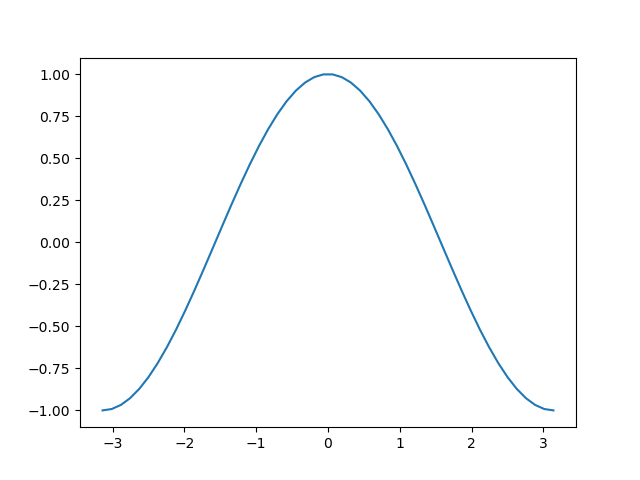
\includegraphics[width=0.7\textwidth]{./data/sen}
%   \caption{Esboço do gráfico da função $y=\sen(x)$ no intervalo $[-\pi,\pi]$.}
%   \label{fig:sen}
% \end{figure}

% Gráficos bidimensionais podem ser criados com a função \lstinline+plt.plot(x,y)+, onde \lstinline+x+ e \lstinline+y+ são \lstinline+arrays+ que fornecem os pontos cartesianos $(x_i, y_i)$ a serem plotados. Por exemplo,
% \begin{lstlisting}
% >>> import matplotlib.pyplot as plt
% >>> x = np.linspace(-np.pi, np.pi)
% >>> y = np.cos(x)
% >>> plt.plot(x,y)
% [<matplotlib.lines.Line2D object at 0x7f99f578a370>]
% >>> plt.show()
% \end{lstlisting}
% produz o seguinte esboço do gráfico da função $y=\sen(x)$ no intervalo $[-\pi,\pi]$. Consulte a Figura \ref{fig:sen}.


% \begin{obs}
%   Matplotlib é uma poderosa ferramenta para a visualização de gráficos. Consulte a galeria de exemplos no seu site oficial
%   \begin{center}
%     \url{https://matplotlib.org/stable/gallery/index.html}
%   \end{center}
% \end{obs}

% \begin{exr}
%   Crie um esboço do gráfico de cada uma das seguintes funções no intervalo indicado:
%   \begin{enumerate}[a)]
%   \item $y = \cos(x)$, $\left[0, 2\pi\right]$
%   \item $y = x^2 - x + 1$, $[-2, 2]$
%   \item $y = \tg\left(\frac{\pi}{2}x\right)$, $(-1, 1)$
%   \end{enumerate}
% \end{exr}

\bibliography{main}
\addcontentsline{toc}{section}{Referências Bibliográficas}

\end{document}
